% vim: ts=4 sts=4 sw=4 tw=80
\chapter{无所不能的 Vim}
\label{chap:vim_can_do_everything}
\marginpar{201}

据说 Vim 可以做任何事情, 虽然这可能不是真的, 但 Vim 的确可以完成许多读者根本
想都不会想到的事情.

在这一节, 我们将会介绍一些原来需要通过 Vim 脚本, 或外部工具才能完成的的事情.

这一节讨论的内容涵盖了游戏, 邮件客户端, IRC 即时聊天, 与集成开发环境的设置.

\section{Vim 游戏}
\label{sec:vim_games}

虽然 Vim 只是一个文本编辑器, 但仍然有很多人开发了大量的脚本, 来让 Vim 完成
其他一些非编辑任务, 其中包括可以直接在 Vim 中玩的小游戏. 这些小游戏不是那些
类似于 ``20 个小问题'' 那样的文本类游戏, 而是带有图形界面的. 这些图形界面
并不完美, 因此它们是用 ASCII 字符组成的界面, 但对于游戏来说已经足够了.
\marginpar{202}

\subsection{生命游戏}
\label{subsec:game_of_life}

第一个要介绍的游戏严格说来, 并不能算作游戏, 但是仍然值得说一下. 生命游戏 (
The Game of Life) 通常被人称为无玩家游戏, 因为这个游戏并不需要玩家参与, 只需
要静静地看着就行. 游戏是一个非常简单的人工智能, 用来模拟细胞的演化. 细胞要
遵守下面几条规则:
\begin{enumerate}
	\item 在一个活的细胞周围, 如果活细胞数少于两个, 则这个细胞会由于孤独而
		死去
	\item 在一个活的细胞周围, 如果活细胞数多于三个, 则这个细胞会由于拥挤而
		死去
	\item 在一个活的细胞周围, 如果活细胞数是两个或三个, 则这个细胞会继续存
		活下去
	\item 在一个死的细胞周围, 如果活细胞数是三个, 则这个细胞会复活
\end{enumerate}

1996 年, 一个自称为大胡子艾丽 (Eli the Bearded) 的人开发了一个 Vim 脚本, 该
脚本实现了生命游戏. 脚本的运行速度并不是非常快, 仅仅是为了阐明游戏的原理.
对于大多数人来说, 这个游戏非常的枯燥, 但是对于生命游戏迷来说, 这是个非常有趣
的实现.

可以到下面这个网址下载生命游戏的 Vim 脚本:
\url{http://www.vanhemert.co.uk/vim/vimacros/life1.vim}.

\subsection{贪吃蛇}
\label{subsec:nibbles}

1986 年, 笔者拥有了第一台 PC, 这台 PC 上只有一个游戏可以玩 --- 贪吃蛇. 笔者
花了很长时间玩这个游戏, 游戏的内容是控制一条小蛇的爬行, 有很多个关卡, 在每个
关卡中, 小蛇都要吃完一定数量的方块后才能过关, 随着方块的增多, 小蛇身体的长度
也在加长. 规则是小蛇不能穿越边界, 也不能穿越自己的身体.

2004 年, Hari Krishna Dara 重新用 Vim 脚本实现了这个游戏. 虽然他的游戏只包含
了很少的关卡, 但是只要用户需要, 就可以添加关卡. 虽然游戏在运行时需要不停地打
印文本, 但是看起来非常得流畅.
\marginpar{203}

\begin{center}
    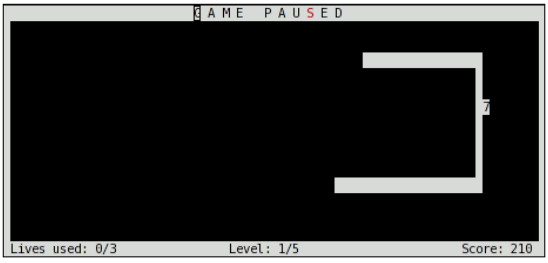
\includegraphics[scale=0.6]{./images/page203-1.png}
\end{center}

脚本的下载地址是 \url{http://www.vim.org/scripts/script.php?script_id=916}.

\subsection{魔方}
\label{subsec:rubik_s_cube}

% FIXME: 字母 o 本来有个双引号重音
1974 年, 匈牙利雕刻家兼建筑学教授 Erno Rubik 发明了一个由 27 个小方块组成的
魔方. 魔方的每一面分别涂上了一种不同的颜色. 如果试图旋转魔方, 那么魔方的颜色
就会变乱, 游戏的目标就是把一个弄乱了的魔方还原成最初的样子.

在 Rubik 发明了魔方的 30 年后, 2005 年, Olivier Vermersch 用 Vim 脚本开发了一
个魔方游戏. Vim 版的魔方同样会让玩家花费几个小时的时间, 把魔方复原.

\begin{center}
    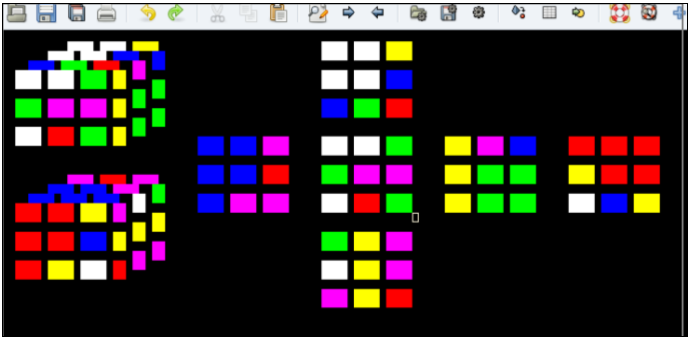
\includegraphics[scale=0.6]{./images/page203-2.png}
\end{center}

2004 年, Charles E. Campbel 重新用 Vim 脚本实现了这个游戏, 用户可以在一个空白
缓冲区中布置一个雷区. 游戏拥有多级难度, 即使用户可以轻易地通过较容易的关卡,
但是当难度上升时, 游戏会让玩家感到非常得头疼.

\marginpar{204}
游戏的使用方法与脚本的下载地址是
\url{http://www.vim.org/scripts/script.php?script_id=1271}

\subsection{井字棋}
\label{subsec:tic_tac_toe}
应该有很多小孩玩过井字棋 (Tic-Tac-Toe) 这个游戏.

1996 年, Kevin Earls 用一系列宏命令在 Vim 中实现了这个游戏, 游戏双方分别是人类
玩家和 Vim.

\begin{center}
    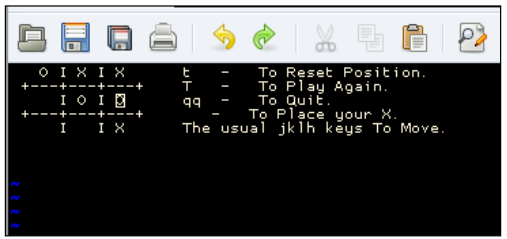
\includegraphics[scale=0.8]{./images/page204.png}
\end{center}

虽然 Vim 的智能不是很先进, 但是想要赢它还是比较困难的.

可以到 Earls 先生的个人主页上下载到游戏脚本, 脚本中包含了游戏的安装与使用方法,
下载地址是 \url{http://www.vanhemert.co.uk/vim/vimacros/ttt.vim}.

\subsection{扫雷}
\label{subsec:mines}

1995 年, 微软在新发布的操作系统 Windows 95 中, 预装了一个称为扫雷的小游戏.
这款游戏混合了数字谜语和一点运气. 玩家的目的是找出雷区中所有的地雷: 或者是
点击没有地雷的方块, 或者是在有地雷的方块上插一把旗子. 方块下的数字表示周围
8 个小方块下的地雷个数. 如果玩家计算出了地雷所在的位置, 就在地雷所在的方块上
插一把小旗子.
\marginpar{205}

2004 年, Charles E. Campbell 用 Vim 脚本重新实现了这个游戏, 游戏包含了多个
难度等级, 脚本的下载地址与使用方法在
\url{http://vim.sourceforge.net/scripts/script.php?script_id=551}.

\subsection{推箱子}
\label{subsec:sokoban}

笔者比较喜欢智力游戏, 也很喜欢推箱子. 游戏玩起来非常简单, 但是游戏本身却可以
非常得难. 游戏的内容是让一个小人把箱子推到指定的位置上. 听起来很简单是吗?
游戏的规则是一次只能推一个箱子, 而且只能推, 不能拉, 因此, 如果把箱子推到角落
中, 那就再也推不动它了, 这时候玩家就不得不重新开始游戏.

2002 年, Mike Sharpe 用 Vim 脚本实现了这个游戏, 游戏的关卡设计来自以前的
Linux 游戏 XSokoban. Mike Sharpe 尽量保持了用户接口的简单, 但游戏玩起来仍然
十分有趣.

\begin{warning}
    XSokoban 游戏可以到这个网址下载:
    \url{http://www.cs.cornell.edu/andru/xsokoban.html}.
\end{warning}

游戏脚本的下载地址是 \url{http://www.vim.org/scripts/script.php?script_id=211}.
\marginpar{206}

\subsection{俄罗斯方块}
\label{subsec:tetris}

最后要介绍的一款游戏是真正的经典 --- 俄罗斯方块, 游戏中会有不同大小与形状的
方块落下来, 玩家的目的是适当地对它们进行排列, 尽量使得每一行都是满的. 俄罗斯
方块是前苏联人 Alexey Pajitnov 在 1985 年发明的, 在这之后, 几乎每个平台都实现
了这个游戏, 而且产生了数以百计的变种.

\begin{center}
    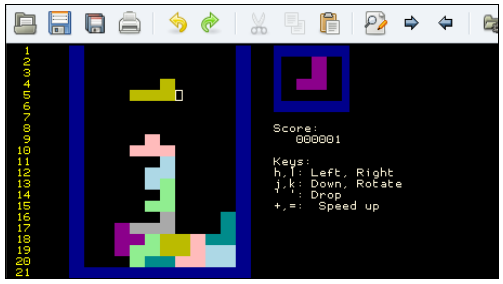
\includegraphics[scale=0.7]{./images/page206.png}
\end{center}

2002 年, Gergely Kontra 用 Vim 脚本实现了这个游戏, 游戏拥有不同的模式, 还可以
记录以前得过的最高分.

脚本的下载地址与使用方法在
\url{http://www.vim.org/scripts/script.php?script_id=172}.

\section{集成开发环境}
\label{sec:programmers_ide}

在书中笔者几次提到, Vim 可以帮助程序员完成很多事情, 从我个人来说, 几乎所有的
编程工作都是用 Vim 完成, 但有时候会听到其他程序员说: ``这么原始的编辑器你是怎
么用的?'', ``没有了集成开发环境, 你是怎么编程的?''. 其实, Vim 同样可以提供集
成开发环境.

首先来看一下集成开发环境应该提供哪些功能.
\marginpar{207}

一个典型的集成开发环境, 比如 Microsoft Windows Visual Studio\textregistered,
包括了下面这些组件:
\begin{itemize}
    \item 支持自动缩进, 语法高亮, 自动补全的编辑器
    \item 集成的编译器, 如果编译出错, 可以直接跳转到出错的地方
    \item 集成的调试器
    \item 文件浏览器
    \item 项目浏览器
    \item 标签浏览器, 通过它可以快速查看变量, 函数, 方法, 类
    \item 支持在文件间, 或定义间快速跳转
    \item 可能还集成了版本控制系统
\end{itemize}
那么, Vim 是否支持上面所说的全部特性呢? 现在我们逐条分析各个特性, 看一下 Vim
如何才能支持它们.

第一条是显而易见的, Vim 本身就是一个功能丰富的编辑器.

第二条是编译器的集成. Vim 通常用于编程工作, 因此它本身就支持编译器集成. 对
常见的编程语言来说, 和编译器集成相关的设置在 Vim 中本来就是设置好了的. 如果
不是, 可以用下面的方法查看如何设置它们:
\begin{vimcode}
:help compiler
\end{vimcode}
编译器集成通常会用到另一个功能: quickfix 列表. 当出现编译错误时, 程序员可以通
过这个列表跳转到出错的代码, 在各个错误之间前进或后退, 修正错误, 然后重新编译.

关于 quickfix 列表的更多信息, 可以查看:
\begin{vimcode}
:help quickfix
\end{vimcode}

下一条是集成的调试器. 和前一条不同的是, 对调试器的支持并不是 Vim 的标准特性.
但是有几个脚本可以帮助 Vim 集成调试器. 如果是 Linux, 可以用 VimDebug, 这个脚
本可以让 Vim 集成 gdb (C/C++ 调试器), jdb (Java 调试器), pdb (Python 调试器),
以及 Perl 调试器. 脚本的下载地址是
\url{http://www.vim.org/scripts/script.php?script_id=663}.
\marginpar{208}

另外一个功能更加丰富的调试器集成是 Clewn, 它集成了 gdb 调试器与 Vim, 支持调
试器的所有功能, 它甚至还支持远程调试. Clewn 的下载地址是
\url{http://clewn.sourceforge.net}.

再下一条是文件浏览器. Vim 本身就带有一个文件浏览器, 不过有一个脚本可以让文件
浏览器与集成开发环境更加搭配, 这个脚本是 VtreeExplorer. VtreeExplorer 不仅可
以浏览文件, 还可以把目录按照树状结构显示出来, 树的结点可以打开或折叠. 脚本的
下载地址是 \url{http://www.vim.org/scripts/script.php?script_id=184}.

接下来是集成开发环境的项目管理部分. 项目浏览器必须支持文件与项目的关联, 这样
的话, 当用户打开某个项目时, 项目内的所有文件就可以同时被打开. 如果用户用的是
Gvim, 就可以用 ProjMgr 脚本. ProjMgr 创建一个菜单项, 该菜单项包含了一张可用
项目列表, 除此之外, 它还可以创建新项目. 脚本的下载地址是
\url{http://vim.sourceforge.net/scripts/script.php?script_id=279}, 控制台版
本的下载地址是 \url{http://www.vim.org/scripts/script.php?script_id=69}.

对于标签浏览器, 有两种解决办法, 其中之一是执行标签名, 函数名, 和其他名字的
补全命令, 然后逐一浏览, 另一种办法是将所有可用的标签列在一个单独的窗口中, 为
了创建这样一个窗口, 笔者推荐 TagList 脚本. 只要是 Ctags 程序支持的编程语言,
TagList 都支持. 脚本会创建一个窗口, 这个窗口列出了所有的定义, 函数, 方法, 和
类, 不仅浏览方便, 还可以快速跳转到声明标签的地方. TagList 的下载地址是
\url{http://vim-taglist.sourceforge.net}.
\marginpar{209}

\begin{center}
    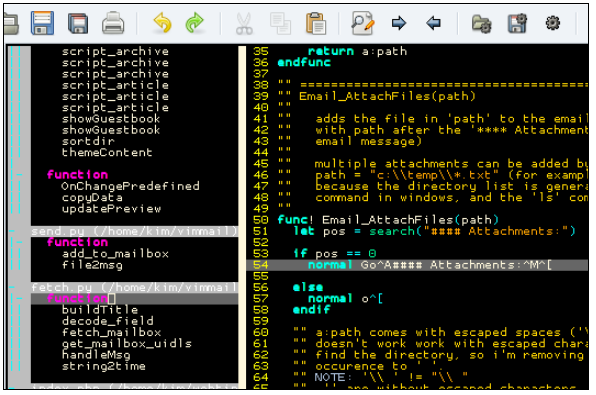
\includegraphics[scale=0.6]{./images/page209.png}
\end{center}
Vim 本身提供了两个命令: \texttt{gf} 与 \texttt{gd}, 分别用来跳转到标签所在
的文件与声明标签的地方, 通过这两个命令的帮助, 用户可以在文件中快速地移动.

最后要谈到的是版本控制系统, 比如 CVS, SVN 和 Perforce. 版本控制系统的集成同
样可以通过脚本来实现. 对于前面提到的三个版本控制系统, 笔者推荐以下几个脚本:
\begin{itemize}
    \item CVS 与 SVN 相关的脚本在
        \url{http://www.vim.org/scripts/script.php?script_id=90}
    \item Perforce 相关的脚本在
        \url{http://vim.sourceforge.net/scripts/script.php?script_id=240}
\end{itemize}

用来组装集成开发环境的各个组件都已经准备好了, 我们现在所要做的就是把它们都
集成起来. 可能有用户怕麻烦, 不想自己动手完成最后一步, 不用担心, 已经有其他人
帮你做好了. 比如 Vim JDE (Just a Development Environment), 它集成了上面提到
的所有脚本, 对 Java, C/C++ 程序员来说, 这是一个功能丰富的集成开发环境. Vim JDE
的下载地址是 \url{http://www.vim.org/scripts/script.php?script_id=1213}.
\marginpar{210}
